\documentclass[doc,12pt]{apa}        % use: 'man' for submission type; 'jou' for
                                % journal type, and 'doc' for typical latex
                                % but with figures inline with text
\usepackage{geometry} 
%\geometry{a4paper} 
\usepackage[parfill]{parskip}   % paragraphs delimited by an empty line

\usepackage{graphicx} 
\usepackage{amssymb}            % no idea what this does...
\usepackage{epstopdf}           % no idea what this does...
%\usepackage{gensymb}            % no idea what this does...

\usepackage{setspace}

\DeclareGraphicsRule{.tif}{png}{.png}{`convert #1 `dirname #1`/`basename #1 .tif`.png} \setcounter{secnumdepth}{0}  % no idea what this does...

\usepackage{apacite}
%%%%%%%%% END HEADER %%%%%%%%%

\title{Rewards are categories.} 
\author{Erik J. Peterson} \affiliation{Dept. of Psychology \\ Colorado State University \\ Fort Collins, CO} 

%%%%%%%%%%%%%%%%
\begin{document} 
%%%%%%%%%%%%%%%%
\maketitle
\doublespacing

\section{Chapter 3 -- fMRI analyses} % (fold)
\label{sec:task_and_models}
\subsection{In acquisition}
\label{sub:acquired}
fMRI data was acquired at the Intermountain Neuroimaging Consortium (INC) facility located at the University of Colorado at Boulder.  All 18 right-handed participants were be pre-screened for the typical fMRI exclusion factors (e.g. metal implants, mental disorders, etc).  Two sets of high resolution anatomical data were acquired. \emph{TODO rest of scan details, cover both localizers and ana}

Following DICOM to nifiti-1 (4D) conversion using dicom2nii (\url{http://www.mccauslandcenter.sc.edu/mricro/mricron/dcm2nii.html}), each dataset was then subjected to the following preprocessing pipeline, carried out in SPM8 using that program's batch mode (\url{http://www.fil.ion.ucl.ac.uk/spm/software/spm8/}).  For complete code see, \url{https://github.com/andsoandso/fmri/tree/master/catreward/spm\_m}).  Anatomical data (MPRAGE) was first segmented in white and grey matter regions \cite{Collignon:1995p9347}.  Based on these segments, parameters necessary for normalization into T1 MNI-352 (1 $mm$) space were calculated.  Anatomical data was then resampled from 1.27 to 1.00 $mm^3$ using fourth degree $\beta$-splines and finally normalized into MNI space.  Normalization had two steps.  The first is a Bayesian 12-parameter affine transformation \cite{Ashburner:1997p9348}.  The second is a set of nonlinear deformations, using a 1127 parameter discrete cosine transform \cite{Ashburner:1999p9350}. 

Movement regressors for all functional volumes were calculated.  No participant moved more than 1.5 $mm$. Functional data was then slice-time corrected, using slice 13 (the middle slice from the descending acquisition) as the reference. Data was then coregistered with the pre-processed (native-space) anatomical data \cite{Collignon:1995p9347}, resampled to 3 $mm^3$ again using fourth degree $\beta$-splines, and normalized into MNI space using the anatomically-derived parameters above.  Finally, the functional data was spatially smoothed using a 6 $mm$ FWHM Gaussian, though a copy of the un-smoothed data was retained for the ROI analyses.  Each voxel's time course was also low-pass filtered (using finite impulse response model, with a cutoff at 0.008 Hz, \cite{Kruggel:1999p9351}) prior to regression analysis.  For all whole-brain analyses, the movement regressors were entered into every model as covariates, accounting for any head movement.

All statistical parametric maps presented below were derived from a Random Effects (RFX, or ``second-level'' in SPM8 jargon) analysis, multiple comparison corrected assuming a Gaussian Random Field using the Family Wise Error Rate (FWE) at the $p < 0.05$ \cite{Worsley:1996p9367}, and a minimum cluster size of 4 voxels), that is except for the raw, unthresholded, maps of $t$-values discussed in the next section.

In fMRI (and in time-series analysis in general) there is an intrinsic trade-off between simply detecting a signal in the presence of noise and then estimating the timecourse (i.e. shape) of that signal \cite{Dale:1999p7901,Birn:2002p1777,Liu:2004p2141}.   One way to optimize over both these objectives is to manipulate the trial order, inside a rapid event-related design \cite{Miezin:2000p7924}.  One state of the art method for setting the trial order is a genetic algorithm which uses two (wieghted) loss functions, one for signal detection and one for time-course estimation \cite{Wager:2003p2980}. \citeNP{Kao:2009p7899}, improved on this design, adding in psychological considerations, and greatly improving executation speed and documentation.  As a result, Kao's method was used to optimize trial orders for part 1 and 2, along with the reward category (i.e. grating only) localizer scan.

\subsection{Maps of blobs}
\label{sub:blob}
Whole brain activity for the stimulus-response learning portion of the behavioral experiment (i.e. part 2) was examined first by comparing all trials to the baseline (rest) condition.  This data is presented in two ways.  First is a transparent overlay of the raw $t$-values.  Second is the more typical statistically thresholded contrast image.  The contrast map showed significant ($t$(15) = 6.59, $p< 0.05$) bilateral activity in the cerebellum, insula and anterior cingulate (Figure~\ref{fig:gl}).  Examination of the raw $t$-values confirms that observed significant effects were robust and widespread in their respective regions, but also allows for the analysis of overall and subthreshold patterns of activity.  These raw data suggest near threshold levels of activity in the head of the caudate, ventrol-medial, dorsal lateral frontal cortices as well as (weaker) activity in the occipital lobe (Figure~\ref{fig:raw}).  And indeed in a two-way ANOVA looking for at that interaction between gains and losses significance clusters were observed in head and body of caudate, insula, posterior and anterior cingulate with the posterior activation extending into the precuneus, dorsal lateral (i.e middle frontal) and ventral medial cortex (Figure~\ref{fig:gxl}; $F$(1, 270) = 30.76, $p < 0.05$).  When trials with gains and losses were examined separately, both showed activity in the same areas as when they were combined (not shown).  Losses showed both increases and decreased of the BOLD signal compared to the rest condition, whereas gains exhibited only increases (not shown).

\begin{figure}[tp]
	\fitfigure{f_map_gl_p05}
    \centering
    \caption{Statistical parametric map for all trials in the stimulus-response learning task (i.e. part 2), compared to the rest period.  \emph{Left} is a glass brain, showing all significant clusters mapped down to 3 two dimensional representations.  \emph{Right} is a set of axial slices highlighting strong areas of activity overlaid onto the T1 MNI-352 template.  $Z$ is the height of the axial slice in MNI space.}
	\label{fig:gl}
\end{figure}

\begin{figure}[tp]
	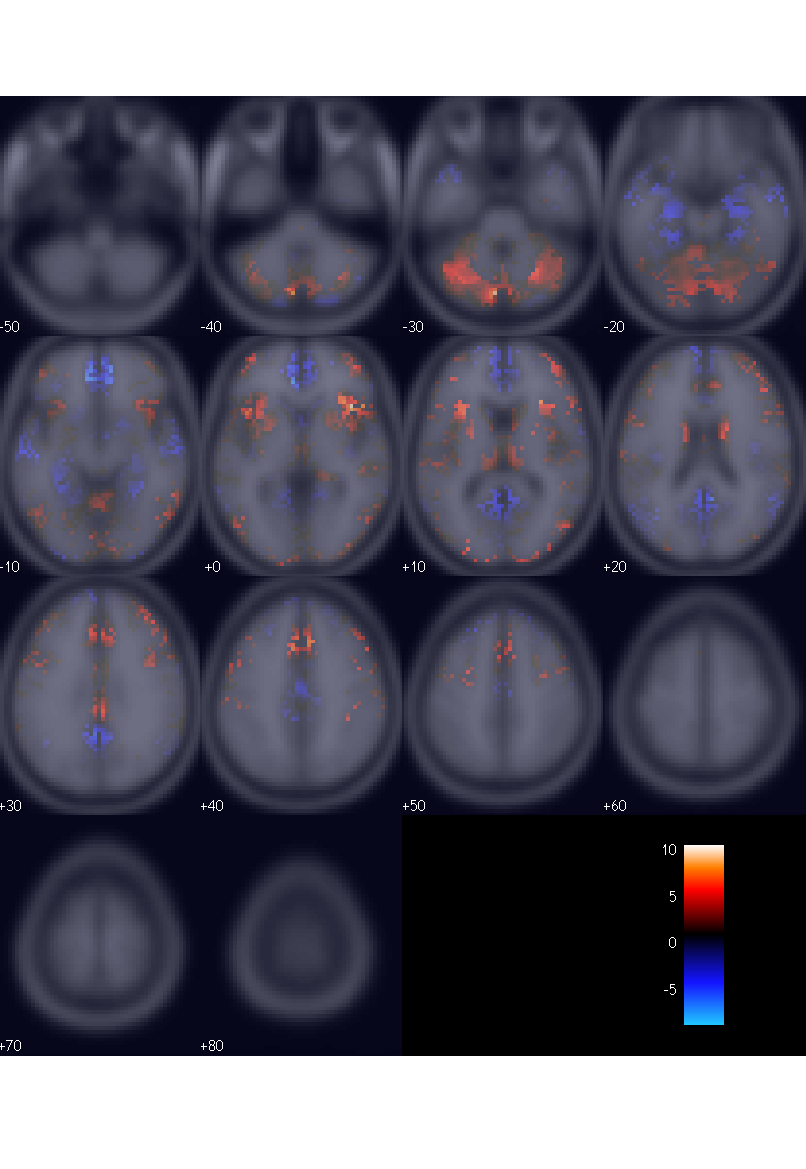
\includegraphics{f_map_gl_raw_t}
    \centering
	\caption{(Raw, that is unthresholded, $t$-values for all trials in the stimulus-response learning task (i.e. part 2), compared to the rest period,  overlaid onto the T1 MNI-352 template.   Each number is the height of the axial slice in MNI space.}
	\label{fig:glraw}
\end{figure}

\begin{figure}[tp]
	\fitfigure{f_map_gxl_p05}
    \centering
	\caption{Statistical parametric map for all trials in the stimulus-response learning task (i.e. part 2) examining the interaction between gains and losses.  \emph{Left} is a glass brain, showing all significant clusters mapped down to 3 two dimensional representations.  \emph{Right} is a set of axial slices highlighting strong areas of activity overlaid onto the T1 MNI-352 template.  $Z$ is the height of the axial slice in MNI space.}
	\label{fig:gxl}
\end{figure}

\subsection{Regions and models}
\label{sub:regoins}
\subsubsection{The right chunks}
\label{subsub:chunks}
Following whole-brain analysis, regions of interest were selected using two methods, that were later compared.  The first employed only regions from the Harvard-Oxford probabilistic anatomical atlas \cite{Desikan:2006p9370}, using the 50\% cutoff.  The second combined anatomical regions with functional clusters isolated using both sets of data collected during the second half of part 1 and from the reward-category localizer outlined above.  Analyses showed that the clustered regions and entire anatomical regions displayed very similar model-fits.  So to limit the complexity of the later analyses, and to possible increase power, functional analyses were dropped.  Only anatomical based analyses are presented here.  Anatomical regions of interest were selected \emph{a priori} based on previous studies of reinforcement and category learning.  Left and right subcortical regions of interest were the dorsal caudate, putamen, ventral striatum/nucleus accumbens, hippocampus, and amygdala.   Bilateral cortical areas were the middle frontal cortex (i.e. dorsal lateral PFC), superior frontal cortex (which contains ventral medial PFC), orbital frontal cortex, anterior and posterior cingulate.

\subsubsection{A Way To Many}
\label{subsub:tomany}
In total there 6 models under evaluation -- the three kinds of similarity adjustment, (``none'', ``exp'', and ``gauss''), with two possible reward codes (``acc'' and ``gl'').  This will expand to include an absolute (positive-only) coding scheme (more on that later), bringing the total to 12 models, with 2 terms of interest (i.e. value and the reward prediction error) that is 24 comparisons.  The are however a number of confounds to our signals of interest, the similarity metrics and the reward codes themselves, the grating parameters, as well as the selected responses.  However as the models are not nested (i.e. they cannot be made identical by simply adding or subtracting parameters (CITE)) and so are not amenable to $F$-tests, the common statistical way to compare fits.  Further complicating the issues is the fact that each of the models is covariate, if not collinear, with the others.  To top it off, none of the three are statistically independent; Reinforcement learning can viewed as a regression of the reward code onto behavioral choices (CITE).  All these factors combined would make statistical testing difficult.  But fortunately finding \emph{the} best model is not the goal.  

The latest recordings of phasic (i.e. reward prediction) activity in the VTA/SNc suggests a complicated reward and prediction error coding scheme (see~\ref{subsub:expectations}), where several separate sets of calculations may be carried out independently \cite{Kim:2006p1063, Matsumoto:2009p7219, Smith:2011p8133}.  The observed BOLD signal is then an aggregate of these many activities, making it possible that more than one of the models under study is correct.  Under this constraint null hypothesis significance tests are not the right choice, model selection is.  Model selection is the process finding a \emph{family} of models/variates that best predict a given dataset \cite{Rao:2001p9457}, with most techniques trying to wisely balance parsimony with increasing fit (i.e. bias versus variance \cite{Geman:1p9469}).  Unfortunately most model selection techniques require assumptions our models cannot meet (e.g. requiring statistical independence).  The few that can tend to be complex recent statistical inventions and rather than navigate the those troubled and unproven waters, I took a simpler approach.  

A score (AIC, Akaike Information Criterion \cite{Akaike:1974p9530}) was assigned to each of the models/codes for every participant and region of interest.  Based on the average score across participants normalized based on the non-parametric (boxcar) model.  The absolute AIC score will vary by participant, but only the relative values are of interest.  Normalization based on the boxcar model, which serves somethings like a null hypothesis, provides a way to cast each participant's fits into relative terms suitable for averaging.  Using the normalized average score each model's performance was then ranked by subtracting each score from the best (lowest) score \cite{Anderson:2000p9475}.  The set of scores that accounted for 95\% of the total possible information were retained \cite{Anderson:2000p9475}.  The retained set was then transformed to Akaike Weights, a way to compare the conditional probabilities of each model being true \cite{Wagenmakers:2004p9472}.

\subsubsection{Information on (Akaike's) Information}
\label{subsub:way}
AIC is a measure of loss; how much information is lost by substituting the model for the true distribution, i.e. the data.  The lower the AIC score, the better the model.  Unlike both the null hypothesis tests, and Bayesian measures, AIC based methods do not seek to find \emph{a} truth, but instead serve to rank models.  It offers then only relative insight, and is unable to make any claims about absolute significance.  Significance is a separate question, one I'll return to later.  Besides this limitation, AIC has some significant advantages. Five reason are reviewed below.

One, unlike maximum-likelihood AIC is designed to a be parsimonious score.  It penalizes for additional parameters.  It may therefore choose a overall worse model (as measured by likelihood of mean squared error) over a better but more complex one. This is the essence of Occam's razor\footnote{Famously and pithily expressed as, ``Entities are not to be multiplied beyond necessity''.}. 

Two, it fits with the process of science.  When designing an experiment it is rare that there are only two possible outcomes, instead typically there are several competing hypothesis, some of which may not be mutually exclusive.  AIC's focus on relative differences, and evidential weights meshes perfectly with the idea of multiple working hypotheses \cite{Burnham:2004p9621}. 

Three, truth can remain elusive.  A common alternative to AIC is BIC, the Bayesian Information Criterion.  Like AIC, it is derived from the log-likelihood of a model, however its derivation requires a rather strict (and often unrealistic) assumption -- that the true model is among the candidates \cite{Forster:2000p9623}.  And while it may be philosophically debatable whether any mathematical model can \emph{completely} describe reality, in this study it is a known fact that my models are incomplete.  The reinforcement learning literature contains several findings I (or anyone) can't yet account for (see the \emph{Introduction} for a review).  

Four, AIC values are easily interpretable once they're transformed to Akaike Likelihoods or Weights\footnote{
    Likelihood for model $k$ among $K$ working hypotheses/models is given by $L_k = e^{-0.5({AIC}_k - {min}_{K}{(AIC)})}$, which is then normalized, becoming an Akaike Weight by $w_k = L_k / \sum\limits_{k=1}^K L_k$ \cite{Burnham:2004p9621}.}.  The likelihood is simply the likelihood the model is correct (based on the information loss associated with it), while the Akaike Weights are just normalized likelihoods.  As the Weights sum to one, the conditional likelihood of one model compared to another is just the ratio of their weights \cite{Burnham:2004p9621}.  For example, if the conditional likelihood of model A over model B is $w_A/w_B$.  That is, the likelihoods and Akaike Weights are intrinsically measures of effect size \cite{Anderson:2000p9475,Forster:2000p9623}.  Despite the fact that it is often used to express the likelihood of correctly rejecting the null hypothesis, the $p$ value is not a measure of effect, as $p$ is contingent not just on effect size but on sample number.  
    
    Five, AIC has a history with models of categorization. \citeNP{McKinley:1996p9532,Maddox:2001p9533}, among several others, used AIC to compare behavioral results to several alternative models of categorization.  

\subsubsection{F-them}
\label{subsub:F}
AIC ranks offer no information on significance, in the familiar null hypothesis sense, or on the absolute fit of the model.  I addressed both of these in a series of $F-tests$ run prior to AIC analysis.  These (fixed-effect, across participant) ominbus tests asked whether the total set of regression parameters for each linear model (described below) could explain the BOLD time series better than chance, i.e could the null hypothesis (of 0) be rejected.  However in keeping with recommendations of \citeNP{Burnham:2004p9621, Forster:2000p9623}, who argue that as AIC and significance tests are so dissimilar that direct comparison/interaction between them them will be at best misleading, the models are not discarded based on significance.  Instead all models are retained, and later AIC ranked.  The $F$-tests are a separate measure whose results are integrated during interpretation, not during model selection/analysis.

\subsubsection{Code, BOLD, and models.}
\label{subsub:aggregating}
No available fMRI analysis package returns AIC scores (or measures that could be converted to such) and none allow for the efficient (i.e programmatic) analysis of many competing computational models. So I created a roi-focused fMRI data \emph{analysis} tool in Python (v2.7.1) to meet those two needs.  This module, simply named ``roi'', has since been release under the BSD license and is available for download at \url{https://github.com/andsoandso/roi}. It relies on the nibabel library to read the nifiti-1 files  (v1.2.0; \url{http://nipy.org/nibabel}), nitime for timeseries analysis, (v0.4; \url{http://nipy.sourceforge.net/nitime/}) Numpy for generic numerical work (v1.6.1; \url{http://numpy.scipy.org/}), with the GLS function from the scikits.statsmodels module handling the regerssions (v0.40; \url{http://statsmodels.sourceforge.net/}).  Model-to-BOLD fit parameters, as well as other useful metadata, was then extracted and stored in text files suitable for importing into R (v2.15.1; \url{http://www.r-project.org/}).  All plotting and model ranking (as well as the $F$-tests) were carried out in R.  For complete BSD licensed code see, \url{https://github.com/andsoandso/fmri/tree/master/catreward/roi/results}.

\subsection{Model Results}
\label{sub:modelresults}


\newpage
\bibliography{bibmin}
%%%%%%%%%%%%%
\end{document}
%%%%%%%%%%%%%
